\documentclass[11pt,twocolumn]{article}
\usepackage[margin=0.75in]{geometry}
\usepackage{amsmath}
\usepackage{amssymb}
\usepackage{setspace}
\usepackage{graphicx}

\usepackage{color}
\definecolor{deepblue}{rgb}{0,0,0.5}
\definecolor{deepred}{rgb}{0.6,0,0}
\definecolor{deepgreen}{rgb}{0,0.5,0}

\usepackage{listings}

\DeclareFixedFont{\ttb}{T1}{txtt}{bx}{n}{12} % for bold
\DeclareFixedFont{\ttm}{T1}{txtt}{m}{n}{12}  % for normal

% Python style for highlighting
\newcommand\pythonstyle{\lstset{
    language=Python,
    basicstyle=\ttm,
    otherkeywords={self},             % Add keywords here
    keywordstyle=\ttb\color{deepblue},
    emphstyle=\ttb\color{deepred},    % Custom highlighting style
    stringstyle=\color{deepgreen},
    frame=tb,                         % Any extra options here
    showstringspaces=false            % 
}}


% Python environment
\lstnewenvironment{python}[1][]
{
    \pythonstyle
    \lstset{#1}
}
{}

    

\begin{document}

\title{ECE 4750 Lab 1: Iterative Integer Multiplier}
\author{Akshay Dongaonkar (akd54) \& Avinash Navada (abn44) \& Vivek Gaddam (vrg22)}
\maketitle

\section{Introduction}

In many programming algorithms, multiplication is a key step in driving the algorithm towards completion. 
Many digital signal processing algorithms spend most of their time multiplying values. Given our media heavy,
highly connected Internet of Things (IoT), more signals will need to be processed. Therefore, we have synthesized 
an iterative multiplier that supports the mul instruction as defined in the PARCv1 Instruction Set Architecture (ISA).
Eventually, this multiplier will be a module in a fully synthesizable multicore processor.

We implemented two multiply designs: the first is a fixed latency, 34 cycle iterative multiplier while the second is a variable latency
iterative multiplier with bounds of 3 to 34 cycles. While we do not expect much additional overhead on clock frequency
in our variable multiplier, we expect a significant increase in area and energy. Given the technology constraints we face today,
(focus on energy, large die sizes, etc), we expect our variable multiplier to be superior in most implementations. 


\section{Project Management}

\section{Baseline Design}

The baseline design works on the following interface: given a 64 bit message containing our operands, a clock signal,
and required signals to conform to the val/rdy microprotocol, output the lower 32 bits of the multiplication to your consumer.
This interface is shown in figure $1$.
\begin{figure}[b]
\centering
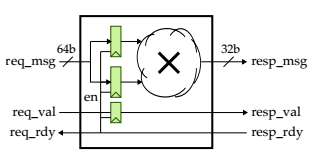
\includegraphics[scale=0.5]{FLmodel}
\caption{Interface for our model. Notice that req/resp,val/rdy signals are part of the val/rdy microprotocol}
\end{figure}
Our algorithm for computing the multiplication consists of repeated adds and shifts on 32 bit values, shown below in pseudocode.
\begin{python}
def imul( a,b ):
    result = 0
    for i in range(32):
        if b & 0x1 == 1:
            result += a
        a = a << 1
        b = b >> 1
    return result
\end{python}
Our implementation follows the structure of this pseudo-code very closely. We have three registers, one for $a$, $b$, and $result$ and we have 
a left shifter and right shifter synthesized by System Verilog. 
We split how the algorithm manipulates these registers along the control-datapath line. 
Our control and datapath logic are placed in \textit{modules} and communicate
via status and control signals. Control signals sent to datapath logic are highlighted in blue in our datapath diagram, shown in figure $2$. 
Control signals are used to select data into our multiplexors %TODO
\begin{figure}[b]
\centering
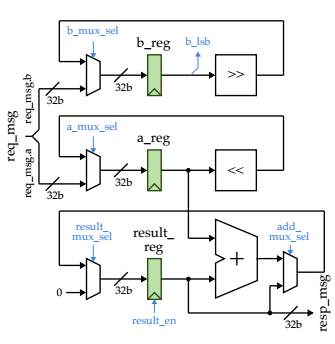
\includegraphics[scale=0.6]{Datapath}
\caption{Datapath Diagram. Again, the structure mimics the pseudocode.}
\end{figure}
There is a single bit status signal sent back to our control module, which is a sample of the least significant bit of the second operand.
This information is used, if you look at the pseudo-code, to determine if a partial sum should be made. Again, we aim to emulate the structure of the code as much as possible.   
 

\section{Alternative Design}

\section{Testing Strategy}

\section{Evaluations and Conclusion}

\end{document}
